\section{Results}\label{sec:results}

\subsection{Full sequence prediction}\label{subsec:full-sequence-prediction}
With different models a variety of results are achieved, but the most important result is that an important baseline for the future development of this kind of systems has been settled down.
For the encoder-only model, in over-fitting with sequence 3, we can obtain a trajectory which is not similar at all after 200 epochs showing no tendency to converge.
\begin{figure}[H]
    \centering
    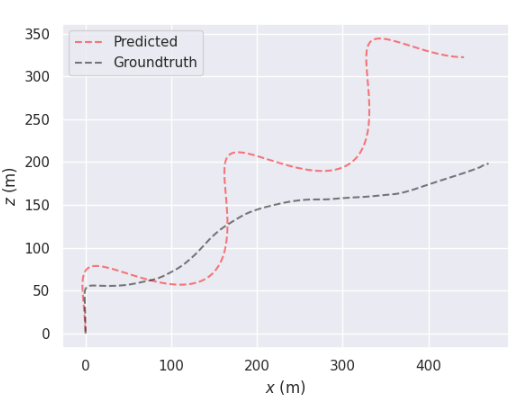
\includegraphics[width=0.8\textwidth]{./images/6_1_trajectory_3_encoder_only}
    \caption{Sequence 3 predicted by encoder-only model}
    \label{fig:trajectory-3-encoder-only}
\end{figure}

After a few trials with encoder-decoder model, which produced some circular trajectories, feeding the \textit{sequence 3} of KITTI (for more details \S~\ref{sec:kitti}) where the first pose of the sequence is considered as origin, we showed that the model (with both 6 and 12 layers of encoder-decoder) is able to learn a single sequence in over-fitting, but fails when trying to over-fit a more complex sequence.
The same model succeeded also in predicting the sequence 7, but failed when we combined the two sequences.
It also fails when we try to over-fit the most complicate sequence, the sequence 0.
\begin{figure}[H]
    \centering
    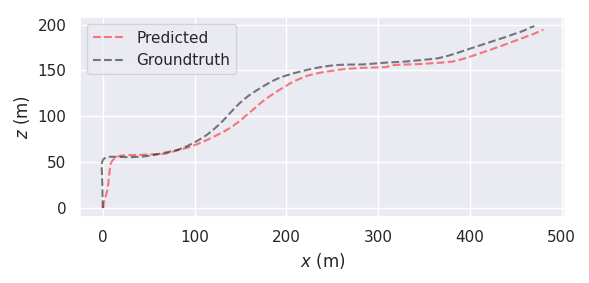
\includegraphics[width=0.8\textwidth]{images/6_1_well_predicted_seq_3}
    \caption{Good prediction sequence 3}\label{fig:well-predicted-seq-3}
\end{figure}
\begin{figure}[H]
    \centering
    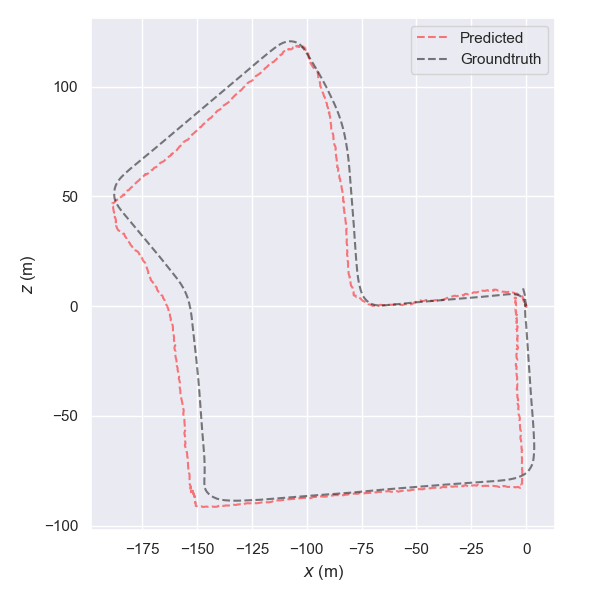
\includegraphics[width=0.8\textwidth]{images/6_1_well_predicted_seq_7}
    \caption{Good prediction sequence 7}\label{fig:well-predicted-seq-7}
\end{figure}
% %**************************************************************

\subsection{Autoregressive models}\label{subsec:autoregressive-model}
We implemented only the encoder-decoder version of the transformer in the autoregressive way, and most of the time the prediction of the network during the training on seq 3 is just a straight line.
So the model is \textbf{not} able to predict the simplest sequence in over-fitting.
The model could not predict any reasonable trajectory, predicting only a linear trajectory as the follow:
\begin{figure}[H]
    \centering
    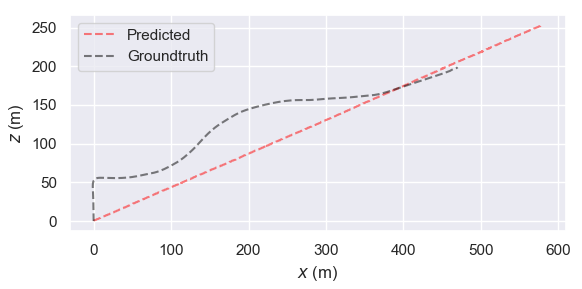
\includegraphics[width=0.8\textwidth]{images/6_1_autoregressive_prediction}
    \caption{Bad prediction sequence 3 of autoregressive model}\label{fig:autoregressive-seq-3}
\end{figure}
Although the model has been trained for more than two hundred epochs, the network cannot understand the goal, and this maybe is due to the loss function.